
%(BEGIN_QUESTION)
% Copyright 2006, Tony R. Kuphaldt, released under the Creative Commons Attribution License (v 1.0)
% This means you may do almost anything with this work of mine, so long as you give me proper credit

{\it RTD-er} brukes ofte i brokretser for å konvertere en temperaturmåling til en spenning:

$$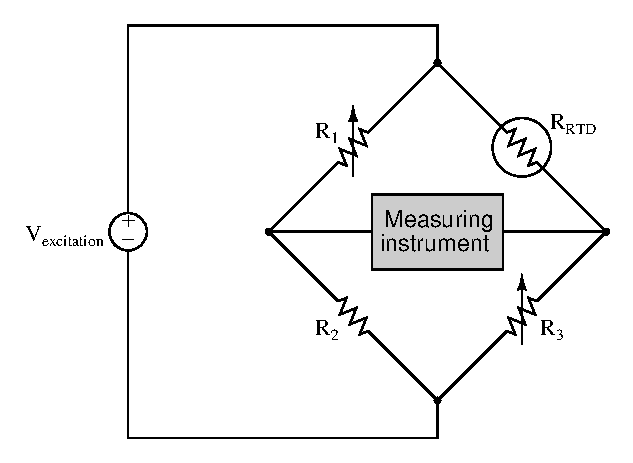
\includegraphics[width=15.5cm]{i00040x01.eps}$$

Anta at broen er balansert når RTD-en er ved sin laveste områdeverdi (LRV).  Identifiser:

\begin{itemize}
\item{} Polariteter på spenningen over alle broresistorer.
\item{} Polariteter på spenningen som måleinstrumentet ser når temperaturen øker mot URV.
\item{} Hvilken variabel motstand ($R_1$ eller $R_3$) som justerer {\it null}.
\item{} Hvilken variabel motstand ($R_1$ eller $R_3$) som justerer {\it spenn}.
\item{} Én elektrisk feil (åpen eller kortsluttet) som gir positivt overområde ($>$ 100 \% temp.) avlesning.
\item{} Én elektrisk feil (åpen eller kortsluttet) som gir negativt overområde ($<$ 0 \% temp.) avlesning.
\end{itemize}

Forklar også {\it hvorfor} du har identifisert null- og spennjusteringsmotstandene som du har:

\vfil 

\underbar{file i00040}
\eject
%(END_QUESTION)





%(BEGIN_ANSWER)

Dette er et vurdert spørsmål -- ingen svar eller hint gis!

%(END_ANSWER)





%(BEGIN_NOTES)


%INDEX% Measurement, temperature: RTD (bridge circuit)

%(END_NOTES)
